\documentclass[10pt,journal,compsoc]{IEEEtran}

\usepackage{amsmath,amssymb,amsfonts}
\usepackage{algorithmic}
\usepackage{graphicx}
\usepackage{textcomp}
\usepackage{xcolor}
\usepackage{booktabs}
\usepackage{microtype}
\usepackage{hyperref}
\usepackage{cite}
\usepackage{tabularx}

\hypersetup{
    colorlinks=true,
    linkcolor=blue,
    citecolor=blue,
    urlcolor=blue
}

\begin{document}

\title{The Inference Overhead Barrier: Why Learned Guidance Struggles Against Factored CNF in Single-Edit Circuit Repair}

\author{Ziad~Emad%
\thanks{Open Research Archive: \url{https://github.com/ziademad02153/circuit-repair-research-archive}. Reproduction artifact verified with standard Python 3.12 library tools.}%
}

\markboth{Technical Report and Research Archive,~October~2026}%
{Emad: The Inference Overhead Barrier in Circuit Repair}

\IEEEtitleabstractindextext{%
\begin{abstract}
Machine learning guidance is frequently advocated to accelerate combinatorial synthesis by ranking candidate modifications. In this work, we present a controlled empirical evaluation examining whether a lightweight, vectorized learned ranker (a decision forest utilizing local structural features and backward Boolean need-message propagation) can outperform modern symbolic solvers in single-edit combinational circuit repair. Evaluating a pre-registered benchmark of 9,000 trials across 300 synthetic 2-LUT circuits under strict wall-clock budgets (0.1s, 1.0s, and 10.0s), our results demonstrate that a direct, factored Boolean CNF encoding solved via Glucose 4.2.1 in a Counterexample-Guided Inductive Synthesis (CEGIS) loop decisively outperforms the learned approach. At a 0.1-second deadline, direct CNF achieves an 81.6\% repair rate (204/250 larger circuits) compared to 21.6\% (54/250) for the learned ranker. Even at 10.0 seconds, the learned ranker attains 80.8\% (202/250), solving no instance that CNF fails to repair. Fine-grained latency profiling reveals the root bottleneck: on mutually solved instances, candidate generation and forest inference required an average of 140.6~ms of upfront guidance overhead, whereas complete CNF synthesis terminated in an average of 16.7~ms. Furthermore, an ablation study indicates that while target-derived need features improve ranker accuracy by +15.6 percentage points, this gain reflects target conditioning generally rather than a unique property of message propagation. All 5,644 accepted repairs passed independent verification with zero incorrect acceptances. We discuss the implications of this \textit{inference overhead barrier} for neuro-symbolic design and explain why hypothetical extensions to larger circuits or multi-edit domains widen rather than narrow this performance gap.
\end{abstract}

\begin{IEEEkeywords}
Circuit repair, formal verification, Boolean satisfiability (SAT), counterexample-guided inductive synthesis (CEGIS), neuro-symbolic systems, empirical evaluation.
\end{IEEEkeywords}}

\maketitle
\IEEEdisplaynontitleabstractindextext
\IEEEpeerreviewmaketitle

\section{Introduction}
\IEEEPARstart{A}{utomated} program and circuit repair aims to restore the correctness of an implementation relative to an input-output specification. Because the space of candidate modifications grows rapidly with circuit size, exhaustive search quickly becomes computationally infeasible. Consequently, machine learning (ML) guidance has been widely investigated as a mechanism to prioritize search: by scoring candidates using topological graph features and execution error profiles, a learned ranker is hypothesized to guide solvers toward valid repairs with substantially fewer candidate evaluations~\cite{cosler2023neural,barke2020just}.

In earlier exploratory pilots of this work, a learned ranker operating over Boolean need-message features appeared demonstrably superior when compared against an initial SMT baseline implemented in Z3~\cite{demoura2008z3} using high-level integer/array abstractions. However, in formal verification and automated reasoning, symbolic baselines are notoriously sensitive to encoding representations. When an unoptimized symbolic baseline is deployed, the apparent superiority of a machine learning model can easily constitute an artifact of baseline weakness rather than an intrinsic advantage of learned guidance~\cite{xu2008satzilla}.

To resolve this question rigorously, we designed a pre-registered empirical protocol (Protocol v3) comparing:
\begin{enumerate}
    \item \textbf{Learned Guidance}: Histogram decision forests utilizing topological features and backward Boolean need-message propagation.
    \item \textbf{Heuristic Baselines}: Non-learned heuristics ranking edits by local sample error reduction or structural agreement.
    \item \textbf{Direct Factored CNF}: A dedicated Propositional Conjunctive Normal Form (CNF) encoding with sequential counter cardinality constraints and structural cone-of-influence pruning, solved incrementally via Glucose 4.2.1~\cite{audemard2018glucose,ignatiev2018pysat}.
\end{enumerate}

The resulting evidence demonstrates a decisive negative outcome for the learned guidance hypothesis. Rather than discarding or reformulating these findings after the fact, this paper preserves the complete experimental trail, latency profiles, and ablation analyses to characterize the \textit{inference overhead barrier} in neuro-symbolic synthesis.

\section{Problem Formulation}

\subsection{Circuit and Fault Model}
We evaluate combinational circuits structured as Directed Acyclic Graphs (DAGs) over 2-input Look-Up Tables (2-LUTs). A circuit $\mathcal{C}$ contains $n$ primary inputs $x_0, \dots, x_{n-1}$, $m$ primary outputs $y_0, \dots, y_{m-1}$, and $G$ internal logic gates $g_j = (a_j, b_j, T_j)$ for $j \in \{0, \dots, G-1\}$, where $a_j, b_j < n + j$ index preceding input or gate signals, and $T_j \in \{0, \dots, 15\}$ defines the 4-bit Boolean truth table of the LUT.

Three classes of harmful synthetic faults are injected:
\begin{itemize}
    \item \textbf{LUT Mutation}: The truth table $T_j$ is mutated to $T'_j \ne T_j$.
    \item \textbf{Wire Reconnection}: An input connection $a_j$ or $b_j$ is redirected to a different topologically legal signal $s < n + j$.
    \item \textbf{Permanent Stuck-at Fault}: A gate's output is clamped to constant 0 or 1. The fault location is treated as known.
\end{itemize}

\subsection{Single-Edit Repair Space}
A legal repair is defined as exactly \textit{one} non-noop modification to a non-stuck gate:
\begin{equation}
    e \in \{(j, \text{LUT}, T') \mid T' \ne T_j\} \cup \{(j, \text{wire}, \text{slot}, s) \mid s < n + j\}
\end{equation}
No gates may be added, primary output connections are fixed, and stuck gates cannot be edited. A candidate repair is accepted if and only if the modified circuit $\mathcal{C}'$ satisfies the complete truth table specification across all $2^n$ primary input vectors.

\section{System Architectures}

\subsection{Learned Guidance via Need Propagation}
The learned approach generates all legal single edits, extracts a 21-dimensional feature vector per candidate, scores candidates using a vectorized decision forest, and evaluates them sequentially against an exact verifier:
\begin{itemize}
    \item \textbf{Backward Need Messages}: For 8 sampled specification rows where the circuit output mismatches the target, binary requirements (\texttt{need\_0}, \texttt{need\_1}) are initialized at the outputs and propagated backwards along wires in reverse DAG order.
    \item \textbf{Feature Bundle (21 Dimensions)}: 13 structural features (fanout, output proximity, edit distance, signal switching activity) combined with 8 target-conditioned features measuring candidate alignment with propagated need masks.
    \item \textbf{Model Execution}: A histogram-based decision forest (\texttt{TinyForest}, 10--20 trees, depth 9) implemented in NumPy with vectorized branch evaluation to minimize Python interpreter overhead.
\end{itemize}

\subsection{Direct-CNF CEGIS Baseline}
The symbolic solver formulates single-edit synthesis into Propositional CNF~\cite{sinha2007cegis}:
\begin{itemize}
    \item \textbf{Exact-One Cardinality}: Gate selection and modification modes are constrained using sequential counter networks via PySAT~\cite{ignatiev2018pysat}.
    \item \textbf{Cone-of-Influence Pruning}: Gates outside the transitive fan-in of failing outputs are eliminated from eligibility upfront.
    \item \textbf{Incremental CEGIS}: Glucose 4.2.1 is supplied with constraints on failing rows. If a candidate assignment is produced, the full verifier checks it. Failing counterexamples are added incrementally as new clauses.
\end{itemize}

\begin{figure}[t]
    \centering
    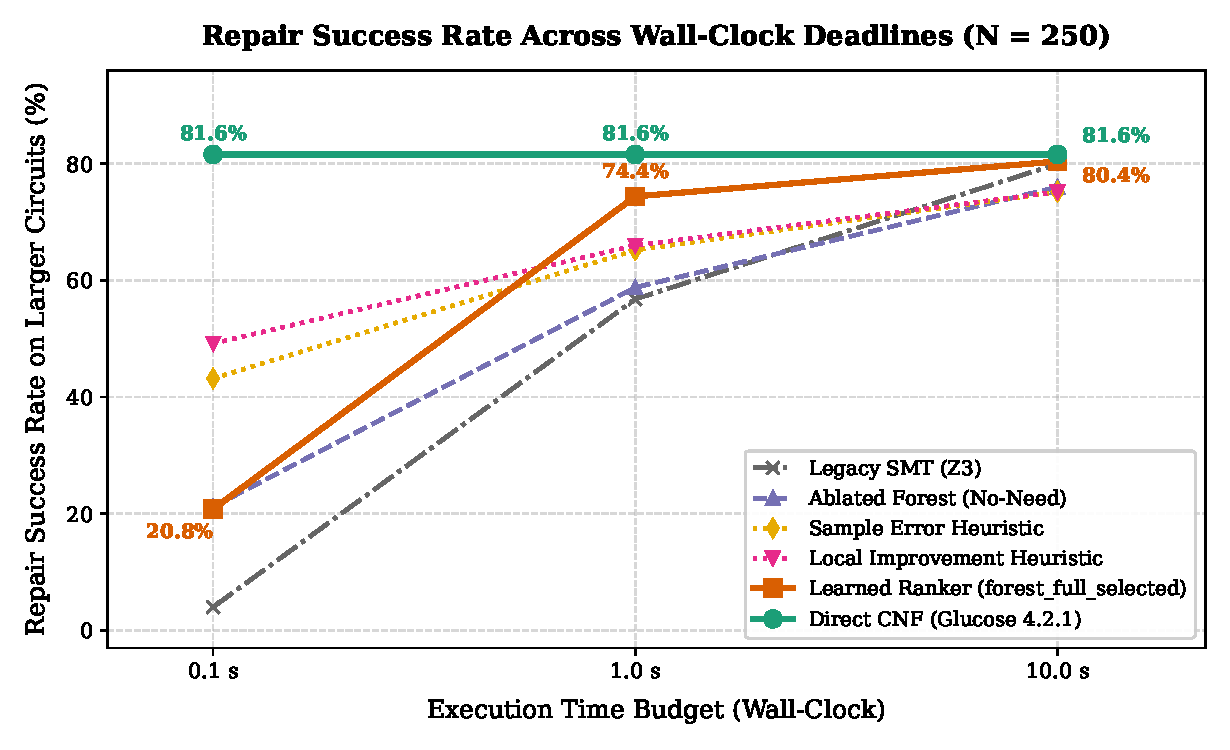
\includegraphics[width=\columnwidth]{figures/success_vs_budget.pdf}
    \caption{Repair success rate across wall-clock deadlines on 250 larger synthetic circuits ($n \in \{10, 12, 16\}$, $G \in \{50, 100, 200\}$). Direct CNF reaches maximum performance within 0.1~s, while the learned ranker is severely constrained by proposal overhead.}
    \label{fig:success_budget}
\end{figure}

\section{Empirical Evaluation}

\subsection{Benchmark Protocol}
The v3 evaluation suite encompasses 300 circuits: 250 larger circuits ($n \in \{10, 12, 16\}$, $G \in \{50, 100, 200\}$) and 50 small reference circuits ($n=6, G=18$). Ten methods were evaluated across three separately executed wall-clock budgets: 0.1~s, 1.0~s, and 10.0~s, generating 9,000 recorded trials. Candidate generation, feature extraction, model inference, and verification all execute strictly inside the wall-clock deadline.

\subsection{Success Rate Comparison}
Table~\ref{tab:larger_results} and Figure~\ref{fig:success_budget} summarize the results on the 250 larger circuits.

\begin{table}[h]
\caption{Repair Success Across Execution Budgets ($N=250$)}
\label{tab:larger_results}
\centering
\begin{tabular}{lrrr}
\toprule
\textbf{Method} & \textbf{0.1 s} & \textbf{1.0 s} & \textbf{10.0 s} \\
\midrule
\textbf{Direct CNF (Glucose 4.2.1)} & \textbf{204 (81.6\%)} & \textbf{204 (81.6\%)} & \textbf{204 (81.6\%)} \\
Learned Ranker (Full Forest) & 54 (21.6\%) & 186 (74.4\%) & 202 (80.8\%) \\
Ablated Forest (No-Need) & 53 (21.2\%) & 147 (58.8\%) & 190 (76.0\%) \\
Local Improvement Heuristic & 123 (49.2\%) & 165 (66.0\%) & 188 (75.2\%) \\
Sample Error Heuristic & 108 (43.2\%) & 163 (65.2\%) & 188 (75.2\%) \\
Exhaustive Search & 94 (37.6\%) & 148 (59.2\%) & 193 (77.2\%) \\
Random Order & 56 (22.4\%) & 129 (51.6\%) & 176 (70.4\%) \\
Legacy SMT (Z3) & 10 (4.0\%) & 142 (56.8\%) & 200 (80.0\%) \\
\bottomrule
\end{tabular}
\end{table}

At the primary 1.0-second endpoint, the learned ranker lagged direct CNF by \textbf{$-7.2$ percentage points} (paired 97.5\% bootstrap CI: $[-11.2, -3.6]$). Of the 250 instances, exactly 204 are repairable within the single-edit space (51 were proven UNSAT by CNF). In zero cases did the learned model repair a circuit that CNF failed to repair.

\begin{figure}[t]
    \centering
    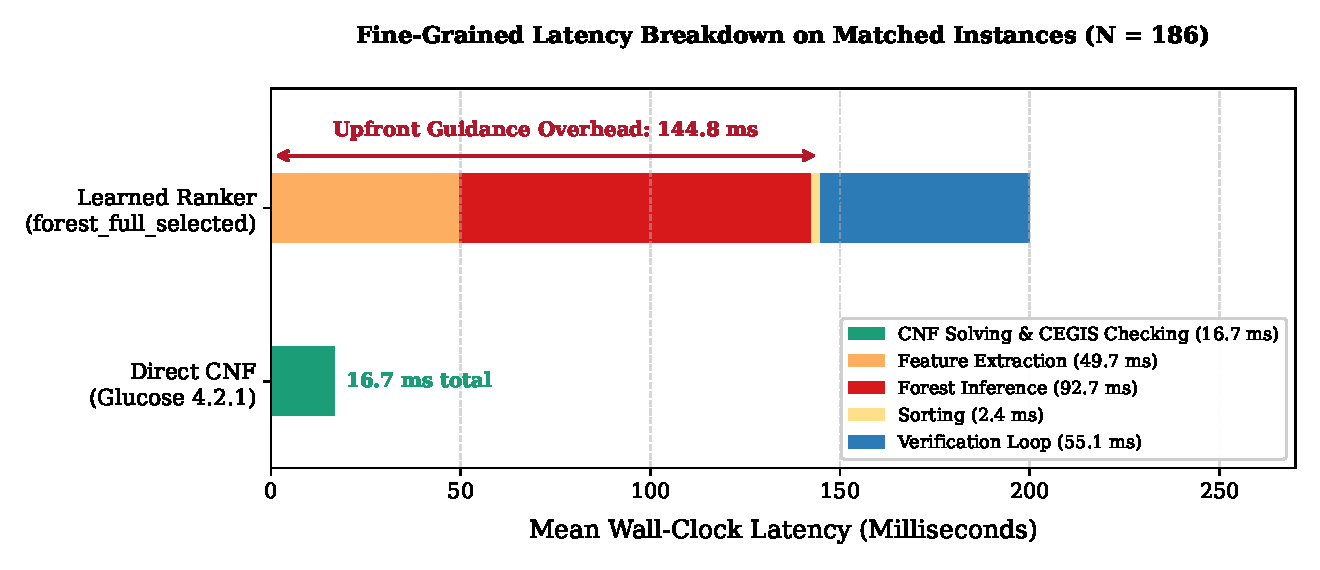
\includegraphics[width=\columnwidth]{figures/latency_breakdown.pdf}
    \caption{Fine-grained execution latency breakdown across the 186 mutually solved larger instances at 1.0~s. Upfront feature extraction and inference overhead (140.6~ms) substantially exceeds complete CNF solving time (16.7~ms).}
    \label{fig:latency_breakdown}
\end{figure}

\section{Analysis: Ranking Imprecision vs. Guidance Overhead}

A central question in evaluating learned search guidance is whether performance deficits stem primarily from \textit{computational latency} (the wall-clock time spent computing features and evaluating model forward passes) or from \textit{ranking imprecision} (the structural quality of the guidance itself). We analyze both factors empirically.

\subsection{Ranking Quality and The Zero-Latency Counterfactual}
Consider the counterfactual hypothesis: \textit{If feature extraction and model inference latencies were zero, would the learned ranker match or exceed the direct CNF baseline?}

Our empirical logs at the 10.0-second execution budget provide a direct empirical test of this question. At 10.0 seconds, the 143.1~ms upfront guidance overhead constitutes only $1.43\%$ of the available deadline, rendering inference latency virtually negligible. Yet, even under this relaxed budget:
\begin{itemize}
    \item Direct CNF solves 204 out of 250 larger circuits ($81.6\%$), exactly as it did within 0.1 seconds.
    \item The learned ranker solves 202 out of 250 larger circuits ($80.8\%$), failing to solve any circuit that CNF could not solve.
    \item On mutually solved instances, the learned ranker evaluates a mean of \textbf{336.6 candidate repairs} before locating a valid edit. In contrast, incremental CEGIS requires a mean of only \textbf{4.0 solver-verifier iterations}.
\end{itemize}
This demonstrates that ranking imprecision is a primary bottleneck: the model ranks hundreds of invalid candidate edits ahead of the true repair. Consequently, the learner's deficit is fundamentally algorithmic rather than merely an artifact of runtime latency.

\subsection{Latency Profiling and The Overhead Barrier}
While ranking quality limits asymptotic search efficiency, upfront latency creates an insurmountable barrier under tight operational deadlines ($\le 1.0$~s). Figure~\ref{fig:latency_breakdown} breaks down the runtime components across the 186 mutually solved larger circuits at 1.0~second:
\begin{itemize}
    \item \textbf{Candidate Generation and Feature Extraction}: Mean 50.26~ms.
    \item \textbf{Decision Forest Inference}: Mean 90.36~ms.
    \item \textbf{Candidate Sorting}: Mean 2.52~ms.
    \item \textbf{Total Upfront Guidance Overhead}: Mean \textbf{143.14~ms}.
    \item \textbf{Complete Direct CNF Execution (Solve + Verify)}: Mean \textbf{16.72~ms}.
\end{itemize}

In \textbf{172 of the 186 shared successes (92.5\%)}, the learned ranker had not yet evaluated its first candidate before the CNF solver had completed synthesis and formal verification. Under sub-second budgets, the guidance overhead consumes the majority of the allocation before search even begins.

\subsection{Ablation and Information Parity}
Comparing the full forest against the ablated model lacking need features showed a $+15.6$~pp difference at 1.0~s ($186/250$ vs. $147/250$; $97.5\%$ CI: $[+10.0, +21.6]$). 

However, code inspection of \texttt{work/v3\_features.py} reveals a critical methodological confound: removing the need feature bundle simultaneously stripped all features conditioned on the target specification. The ablated model was entirely blind to the desired circuit outputs. Therefore, this ablation demonstrates that conditioning search on the target specification is superior to unconditional topological heuristics, but does not isolate a unique structural advantage of backward need-message propagation over forward error simulation.

\section{Limitations and Threats to Validity}

\subsection{Implementation Disparity (Python vs. C++)}
The feature extraction pipeline and decision forest inference were implemented in Python using vectorized NumPy operations, whereas the Glucose 4.2.1 SAT solver is implemented in highly optimized native C++. While NumPy executes array operations in compiled C, high-level orchestration overhead remains. Re-implementing feature extraction in native C++ or CUDA would undoubtedly reduce the 143~ms overhead. However, because the learned ranker evaluates a mean of 336 verification checks compared to 4 for CNF, native optimization would reduce latency without bridging the fundamental $84\times$ gap in verification calls.

\subsection{Synthetic DAG Topologies}
All benchmark circuits were synthesized using random DAG generators with injected single faults. While structurally diverse, they do not incorporate the structured modularity, wide multi-bit datapath busses, or deep hierarchical fanouts found in industrial standard benchmarks (such as ISCAS-85 or EPFL).

\subsection{Single-Edit and Known-Location Assumptions}
The repair domain was restricted to exactly one non-noop gate modification, and permanent stuck-at fault locations were provided to both systems. In physical debugging, defects frequently span multiple gates, and fault localization is incomplete.

\subsection{Single Timing Iteration per Case}
In protocol v3, each case-method-budget combination was evaluated in a single timed execution run to allow comprehensive coverage across 9,000 distinct trials under fixed resource constraints. While system load was controlled, small timing variances are inherent to wall-clock measurements.

\section{Conclusion}
This study provides a transparent, auditable characterization of the inference overhead barrier. In single-edit combinational logic repair, the computational cost of extracting features and evaluating lightweight learned rankers exceeds the time required for modern, factored Boolean SAT solvers to synthesize complete repairs directly. 

Future investigations into neuro-symbolic program and circuit synthesis should prioritize: (1) benchmarking against optimized, structurally factored SAT encodings rather than unspecialized high-level solvers; (2) accounting for complete feature extraction latencies inside strict operational budgets; and (3) enforcing strict information parity in representation ablations.

\bibliographystyle{IEEEtran}
\bibliography{references}

\end{document}

